\begin{document}
\maketitle

\section{简介}
本项目实现了一个网格简化程序。%
能够将输入的OBJ三维模型使用两种算法按照一定的简化比进行简化,%
将简化结果实时显示出来或输出到OBJ文件。%

\section{算法}
\subsection{二次误差度量方法简化}
假定模型中所有平面都是三角形,%
每个三角形满足$n^Tv+d=0$,其中$n=[n_x\ n_y\ n_z]^T$是单位向量,%
$d$是常数。顶点$v=[x\ y\ z]^T$到这个平面距离的平方可以用下式表示:%
\begin{equation}
D^2=(n^T+d)^2=(v^Tn+d)(n^Tv+d)=v^T(nn^T)v+2dn^T+d^2
\end{equation}
此式可以用二次型$Q$来表示顶点到平面距离的平方$D^2$:%
\begin{equation}
Q=(A,b,c)=(nn^T,dn,d^2)
\end{equation}
\begin{equation}
Q(v)=v^TAv+2b^Tv+c
\end{equation}
有性质:
\begin{equation}
Q_1(v)+Q_2(v)=(Q_1+Q_2)(v),(Q_1+Q_2)=(A_1+A_2,b_1+b_2,c_1+c_2)
\end{equation}
通过此性质可以方便地计算顶点到面集合距离的平方和。%
当边$(v_1,v_2)$收缩为$\bar{v}$时,%
收缩代价$Q(\bar{v})=Q_1(\bar{v})+Q_2(\bar{v})$。

计算所有的边的收缩代价并排序,迭代收缩代价最小的边并更新其他边。%

\subsection{改进的二次误差度量方法}
上述算法中边收缩代价的存储和更新计算量大、速度慢。%
改进的二次误差度量方法与上述方法不同,%
改进的算法中通过边收缩代价计算每个面的收缩代价,%
每次收缩时收缩一个面,这样网格的面片数可以连续变化,%
而且可以处理不封闭网格。%
同时使用基于阈值的迭代方式,速度大大提高。%

\section{运行效果}
图形界面显示化简结果的效果如下列图片所示,%
其中左边的是二次误差度量方法简化结果,%
右边的是改进的算法化简的结果。

\begin{figure}[!htbp]
    \centering
    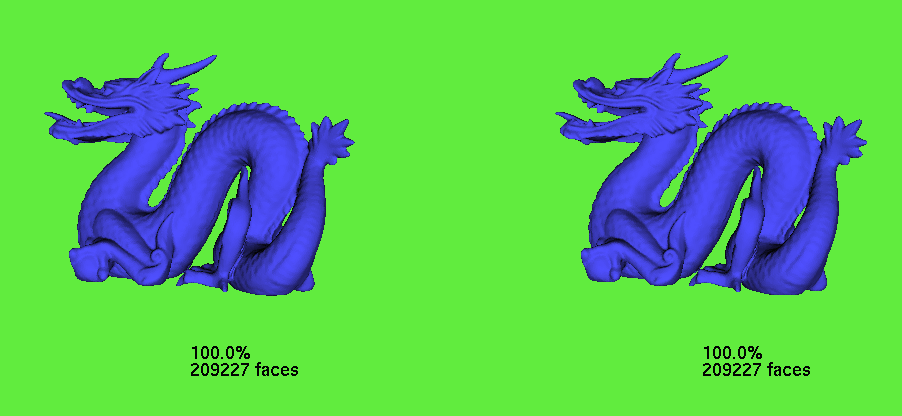
\includegraphics[width=\columnwidth]{100.png}
    \caption{未简化的结果}
    \label{fig:org}
\end{figure}

\begin{figure}[!htbp]
    \centering
    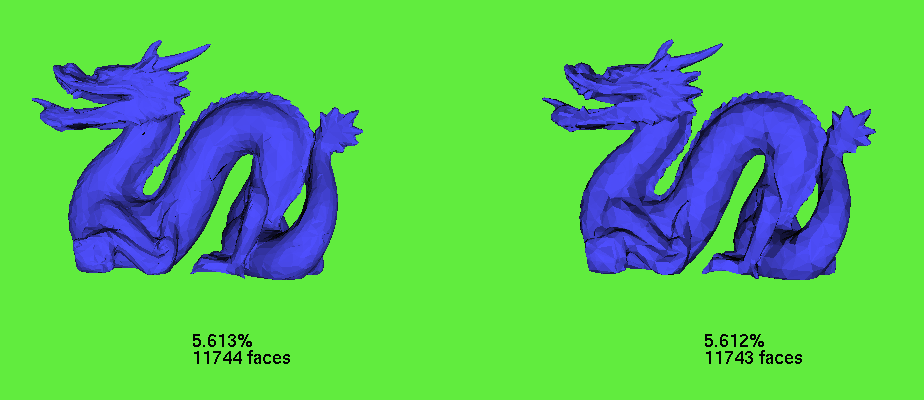
\includegraphics[width=\columnwidth]{5.612.png}
    \caption{简化比为5.6\%时的结果}
    \label{fig:sim1}
\end{figure}

\begin{figure}[!htbp]
    \centering
    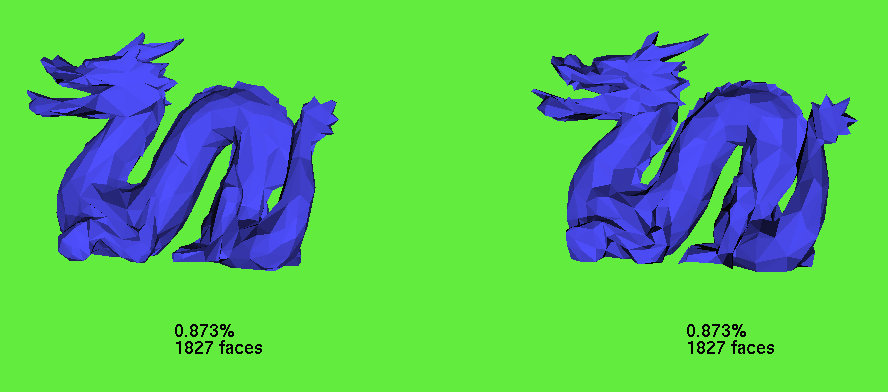
\includegraphics[width=\columnwidth]{0.873.png}
    \caption{简化比为0.87\%时的结果}
    \label{fig:sim2}
\end{figure}

\begin{figure}[!htbp]
    \centering
    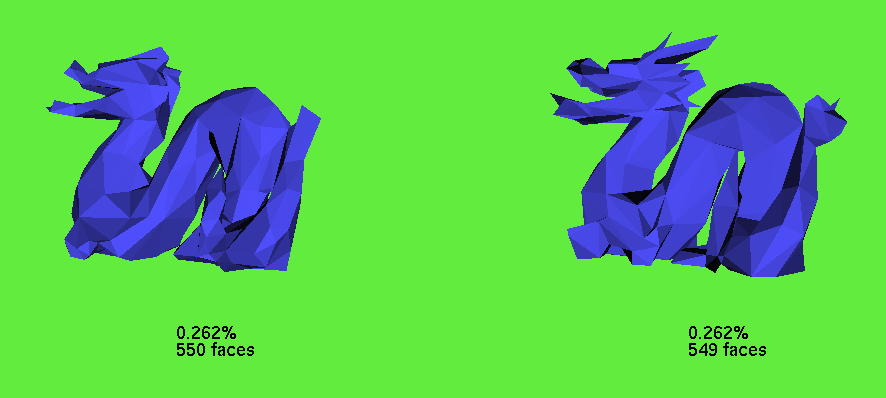
\includegraphics[width=\columnwidth]{0.262.png}
    \caption{简化比为0.26\%时的结果}
    \label{fig:sim3}
\end{figure}

\begin{figure}[!htbp]
    \centering
    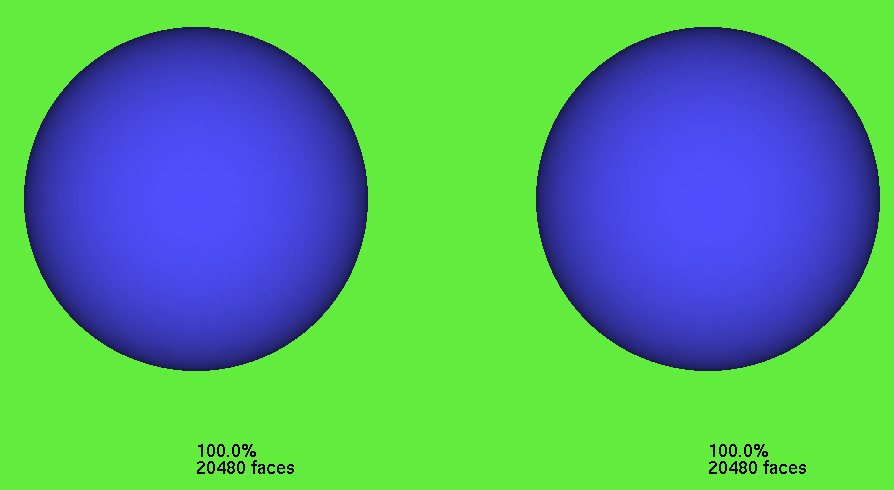
\includegraphics[width=\columnwidth]{100_2.png}
    \caption{未简化的结果}
    \label{fig:org2}
\end{figure}

\begin{figure}[!htbp]
    \centering
    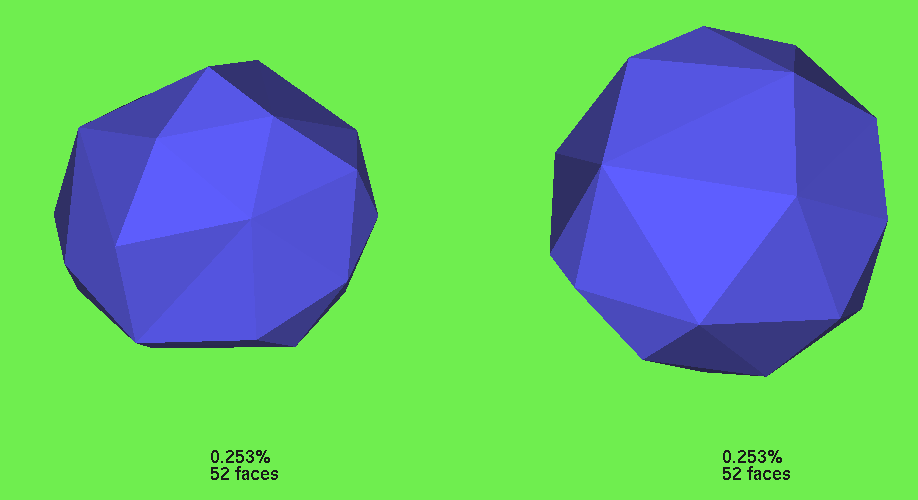
\includegraphics[width=\columnwidth]{0.253_2.png}
    \caption{简化比为0.25\%时的结果}
    \label{fig:sim4}
\end{figure}

从图\ref{fig:sim2}、图\ref{fig:sim3}、图\ref{fig:sim4}中可以明显地看到,%
改进的算法能更好地保留模型的特征。

使用未改进的算法简化图\ref{fig:org}中$209227$个面片的龙模型到$1\%$,%
大约需要2.9秒的时间(单线程,下同),使用改进的算法只需要0.6秒。

\section{源文件}
main.cc 主函数

common.h 通用声明和定义

vector3.h 三维向量类,具有加、减、内积、外积、单位化运算功能

matrix.h 矩阵类,提供矩阵加法功能

triple.h 三元组,类似std::pair,方便程序设计

quadric.h 二次误差度量算法

improved\_quadric.h 改进的二次误差度量算法

parser.h OBJ文件解析类,读取和输出OBJ文件

preview.h 基于OpenGL的显示类

\section{编译和运行}
\subsection{编译}
编译需要OpenGL3.0或以上版本链接库,%
编译器需支持C++11(建议GCC4.8及以上,%
VisualStudio 2012内置MSVC++ 11.0仅部分支持C++11,%
可能不能通过编译)。%
程序中使用了C++11线程库,编译时可能需要设置额外的参数。%

\subsection{运行}
使用图形界面的运行命令为MeshSimplification OBJFILE。

MeshSimplification为可执行文件,%
OBJFILE为OBJ文件。

不使用图形界面的运行命令为MeshSimplification INPUTFILE OUTPUFILE RATIO。

MeshSimplification为可执行文件,%
INPUTFILE为输入OBJ文件,%
OUTPUTFILE为输出OBJ文件,%
RATIO为简化比。

目前OBJ文件仅支持三角形面片,%
不支持纹理、材质、多边形面片语法。%
不支持的语句会被忽略。

\section{开发环境}

Language: C++

Operating System: Linux 3.14.8-200.fc20.x86\_64

Compiler: icpc version 14.0.1 (gcc version 4.8.0 compatibility)

OpenGL: Version 3.0

CPU: Intel(R) Core(TM) i7-3630QM CPU @ 2.40GHz

Memory: Configured Clock Speed 1600 MHz 

源代码在上述环境下编译通过且运行正确,%
本文中测试数据也在上述环境下测得。

\section{参考资料}
\begin{enumerate}[ label={[\arabic*]} ]
\item
孙家广,胡事民.计算机图形学基础教程(第2版)[M].北京:清华大学出版社,2009.8
\item
Garland, M. \& P.S.Heckbert.Surface Simplification Using Quadric Error Metrics[C].Pittsburgh:Carnegie Mellon University
\item
3D GIS.约束条件下二次误差度量简化方法[N/OL].博客园,2007.10.\url{http://www.cnblogs.com/wuhanhoutao/archive/2007/11/10/955004.html}
\item
Spacerat.Quadric Mesh Simplification with Source Code[N/OL].2014.5\url{http://voxels.blogspot.jp/2014/05/quadric-mesh-simplification-with-source.html}

\end{enumerate}

\end{document}
